% !TEX encoding = UTF-8 Unicode

\documentclass[a4paper]{article}

\usepackage{color}
\usepackage{url}
\usepackage[T2A]{fontenc} % enable Cyrillic fonts
\usepackage[utf8]{inputenc} % make weird characters work
\usepackage{graphicx}
\usepackage[table,xcdraw]{xcolor}
\graphicspath{ {Slike/} }

\usepackage{listings}

\definecolor{dkgreen}{rgb}{0,0.6,0}
\definecolor{gray}{rgb}{0.5,0.5,0.5}
\definecolor{mauve}{rgb}{0.58,0,0.82}

\lstset{frame=tb,
  language=C,
  aboveskip=3mm,
  belowskip=3mm,
  showstringspaces=false,
  columns=flexible,
  basicstyle={\small\ttfamily},
  numbers=none,
  numberstyle=\tiny\color{gray},
  keywordstyle=\color{blue},
  commentstyle=\color{dkgreen},
  stringstyle=\color{mauve},
  breaklines=true,
  breakatwhitespace=true,
  tabsize=3
}

\usepackage[english,serbian]{babel}
%\usepackage[english,serbianc]{babel} %ukljuciti babel sa ovim opcijama, umesto gornjim, ukoliko se koristi cirilica

\usepackage[unicode]{hyperref}
\hypersetup{colorlinks,citecolor=green,filecolor=green,linkcolor=blue,urlcolor=blue}


\begin{document}

\title{Optimizacija izvršavanja programa kroz Iterativnu Kompilaciju\\ \small{Seminarski rad u okviru kursa\\Metodologija stručnog i naučnog rada\\ Matematički fakultet}}

\author{Filip Novović, Aleksandar Preočanin, Aleksandar Milosavljević\\ filipn@post.com, preocanin.aleksandar@gmail.com, alemilosav@gmail.com }
\date{14.~april 2017.}
\maketitle

\abstract {
  U ovom radu opisujemo metod \emph{iterativne kompilacije} 
  i motivaciju za njeno korišćenje. Objašnjavamo suštinu ovog pristupa optimizaciji, kao i zbog čega 
  je primenjiv na bilo koju arhitekturu ili algoritamski problem. 
  Dajemo uporedne podatke o brzini izvršavanja 
  iterativno kompajliranih programa sa programima kompajliranim na statički način.
  Zatim, opisujemo neke od čestih tehnika 
  statičke optimizacije petlji i efikasnog korišćenja keš memorije i 
  razjašnjavamo kako nam one mogu biti korisne u iterativnoj tehnici prevođenja programa.
  Otkrivamo kako izabrati najbolje od tih tehnika uz korišćenje najboljih 
  parametara za dati problem i arhitekturu.
  Konačno, upoređujemo potrošnju energije ovakvih programa sa potrošnjom energije statički kompajliranih programa.
}
\tableofcontents

\newpage

\section{Uvod}
\label{sec:uvod}

U poslednjih 30 godina svedoci smo neverovatnog napretka kompjuterskih tehnologija. 
Računari su za veoma kratko vreme prešli put od čuda tehnike koje je dozvoljeno posmatrati isključivo kroz stakleni zid serverske sobe, 
do uređaja čije se korišćenje podrazumeva u svakodnevnom radu čoveka. Broj uređaja koje možemo smatrati računarima se konstantno povećava iz godine u godinu. 
Od mobilnih telefona, preko prenosnih računara, pa sve do pametnih veš-mašina, računari su postali sastavni (vrlo često i centralni) deo uređaja za koje, 
do pre samo par godina, nismo mogli ni da pretpostavimo da će postati ,,pametni''.
\par
Ovaj fenomen eksplozije broja računara i njegovih primena doveo je do nekih logičnih posledica. 
Arhitektura procesora od uređaja do uređaja postala je izuzetno šarolika. Zahtevi za uštedom memorije, procesorskog vremena i energije (struje) postali su primarni na uređajima koji nisu 
(i ne mogu biti) na konstantnom izvoru napajanja. Optimizacija je ponovo postala ključni deo problema u razvoju softvera. 

\par
Sa druge strane postoji velika potražnja za softverom koji rešava raznovrsne probleme, a koji se pritom izvršava na još raznovrsnijim arhitekturama i platformama.
Veliki broj problema koji može biti rešen softverski sa jedne strane i nedovoljan broj razvijaoca softvera sa druge nam govori da je brz razvoj sofvera neophodan kako bi svi problemi 
mogli da se reše u razumnom roku. Način na koji industrija odgovara na taj izazov godinama unazad bio je uopštavanje arhitekture računara koji je omogućio razvijaocima softvera 
da na gotovo isti (ili veoma sličan) način i sa istim alatima i jezicima razvijaju softver za veoma različite platforme. Posledica takvog pristupa je da uopšteni model arhitekture gotovo uvek zanemaruje 
naprednije mogućnosti modernih arhitektura procesora. Korišćenjem samo osnovnih hardverskih funkcionalnosti procesora dolazimo do programa koji su veoma malo (ako uopšte) optimizovani.

\par 
Moderni programski prevodioci uglavnom primenjuju neke statičke tehnike optimizacije, primenjujući različite 
\emph{transformacije} koda koje čuvaju semantičko značenje, kako bi proizveli što optimizovaniji izvorni kod, ali tu nastaju novi problemi. 
Niz transformacija koji daje dobre rezultate na jednoj arhitekturi i za jedan tip algoritamskog problema, 
na drugoj arhitekturi i za drugi tip problema može proizvesti rezultat koji je lošiji od neoptimizovanog rešenja \cite{gheorghita2005iterative}.
Rešenje ovog problema se nazire u konfigurabilnosti redosleda i ulaznih parametara ovih transformacija.
\par
U ovom radu opisujemo jedan pristup optimizaciji u procesu prevođenja koji je nezavisan od platforme i arhitekture. 
Suština ove metode prevođenja je u dodatnom sloju koji se nalazi između izvornog koda i prevodioca. 
Svrha tog sloja je da proizvede optimizovaniji \emph{izvorni k\^{o}d} koji se zatim prosleđuje 
prevodiocu. Kako postoje različiti načini transformacije jednog izvornog koda u drugi, i kako ne postoji jedan statički niz transformacija i njihovih konfiguracija koji bi dao optimalne rezultate za sve probleme i platforme, 
jasno je da odabir transformacija i ulazne parametre tih transformacija moramo naći nekakvom pametnom pretragom. 
Taj proces pretrage parametara nazivamo \emph{,,Iterativna kompilacija''} \cite{kisuki2000iterative}.
\par
Ovaj rad organizovan je na sledeći način. 
U odeljku \ref{sec:transformacije} opisujemo neke od transformacija izvornog koda koje je moguće koristiti pri optimizaciji. 
Koncentrišemo se (naravno) na one transformacije koje su konfigurabilne. Pokazujemo na koji način ove transformacije utiču na performanse i kako se mogu kombinovati. 
U odeljku \ref{sec:pretraga} poredimo različite metode pretrage ulaznih parametara niza transformacija.
U odeljku \ref{sec:performanse} poredimo performanse programa prevedenih na ovaj način kroz različite repere i realne programe, i poredimo potrošnju energije tih programa.
Konačno, dajemo zaključak na osnovu rezultata merenja performansi i potrošnje energije u odeljku \ref{sec:zakljucak}.


\section{Metode transformacija}
\label{sec:transformacije}

Optimizacija kompilatora ima za cilj da minimizuje ili maksimizuje određena svojstva izvršnog koda programa (npr. potrebnu procesorsku energiju) i obično se implementira u obliku niza optimizacionih transformacija. Transformacije su izmene koje se vrše nad kodom kako bi se dobile željene performanse pri njegovom izvršavanju uz uslov da izmenjen kod mora da bude semantički ekvivalentan originalnom. Optimizacija petlji je veoma značajna zato što je procenat vremena koje programi pri izvršavanju provode u petljama veliki. Iz tog razloga ćemo se u ovom poglavlju većim delom koncentrisati na njih.  \\

\textbf{Odmotavanje petlji} (eng. loop unrolling). Koristi se za smanjivanje vremena koje je potrebno za
izvršavanje petlje po cenu povećavanja veličine koda koji joj odgovara. Cilj je da se u petlji
smanji broj instrukcija koje se vezuju za kontrolu toka petlje. Odmotavanje petlji obično ima
veliki doprinos kada u telu petlje postoje naredbe koje su nezavisne, odnosno mogu da se
paralelno izvršavaju. Ovo se ostvaruje pružanjem većeg broja instrukcija hardveru nego u 
slučaju originalnog koda.\\
Primer petlje koja vrši sve iteracije bez odmotavanja:
\begin{lstlisting}

 int x;
 for (x = 0; x < 100; x++)
 {
     delete(x);
 }
\end{lstlisting}
i verzija u kojoj je upotrebljeno odmotavanje:
\begin{lstlisting}
 int x; 
 for (x = 0; x < 100; x += 5)
 {
     delete(x);
     delete(x + 1);
     delete(x + 2);
     delete(x + 3);
     delete(x + 4);
 }
\end{lstlisting}


\textbf{Podela na blokove} (eng. loop tiling). Telo petlje se deli na manje blokove kako bi se osiguralo
da lokalni podaci koji se u njemu koriste ostaju u keš memoriji sve dok ne budu opet bili potrebni.
Doprinos se ogleda u smanjenom broju promašaja keš memorije, kao i energije memorijskog sistema koja
bi bila utrošena na prikupljanje podataka sa alternativnih izvora.\\
Primer koda koji vrši množenje matrica:

\begin{lstlisting}
  int i, j, a[100][100], b[100], c[100];
  int n = 100;
  for (i = 0; i < n; i++) {
    c[i] = 0;
    for (j = 0; j < n; j++) {
      c[i] = c[i] + a[i][j] * b[j];
    }
  }
\end{lstlisting}
i njemu odgovarajuća verzija koja deli prostor iteracije na blokove:
\begin{lstlisting}
  int i, j, x, y, a[100][100], b[100], c[100];
  int n = 100;
  for (i = 0; i < n; i += 2) {
    c[i] = 0;
    c[i + 1] = 0;
    for (j = 0; j < n; j += 2) {
      for (x = i; x < min(i + 2, n); x++) {
        for (y = j; y < min(j + 2, n); y++) {
          c[x] = c[x] + a[x][y] * b[y];
        }
      }
    }
  }
\end{lstlisting}

\textbf{Podela petlji} (eng. loop fission). Telo petlje se deli na dve ili više različitih petlji. 
Doprinos je u ovom slučaju smanjenje broja promašaja instrukcijske keš memorije i stvaranje mogućnosti da se, 
ukoliko su tela novonastalih petlji dovoljno mala, 
koriste baferi petlji (eng. loop buffer\footnote{Bafer petlje je mala, jako brza memorija koja čuva određen broj vremenski skoro korišćenih naredbi. Ukoliko je bafer petlje dovoljno veliki da sadrži sve naredbe tela petlje, onda je potrebno samo jednom uzeti te informacije iz memorije, i to pri prvoj iteraciji \cite{stallings2000computer}}). Negativna posledica podele petlji je povećana potreba za energijom memorijskog sistema usled smanjenja vremenske lokalnosti podataka (eng. temporal locality).\\
Primer petlje u kojoj vršimo dve naredbe:
\begin{lstlisting}
  int i, a[100], b[100];
  for (i = 0; i < 100; i++)
  {
    a[i] = 1; 
    b[i] = 2;
  }
\end{lstlisting}
koju delimo na dve petlje sa po jednom naredbom koje imaju isti opseg:
\begin{lstlisting}
  int i, a[100], b[100];
  for (i = 0; i < 100; i++)
    a[i] = 1;                     
  for (i = 0; i < 100; i++)
    b[i] = 2;
\end{lstlisting}

\textbf{Spajanje petlji} (eng. loop fusion). Predstavlja transformaciju suprotnu podeli petlji. Kombinuje tela dve ili više petlji koje imaju iste
granice u jednu. Ukoliko petlje koje spajamo koriste iste podatke, ovom transformacijom povećavamo
njihovu lokalnost. Smanjenjem broja instrukcija koje se koriste za logiku kontrole toka umanjuje se 
i potrebna ukupna procesorska energija.\\

\textbf{Popunjavanje niza} (eng. array padding) postavlja dimenziju niza na novu vrednost. Niz mora biti lokalna varijabla, a njegova dimenzija konstantna vrednost.

\section{Pretraga ulaznih parametara}
\label{sec:pretraga}
Optimizacione transformacije međusobno imaju različite uticaje na kod. 
Uprkos tome što transformacije koristimo kako bi se u kodu ispoljile njihove pozitivne osobine, 
treba imati u vidu da loše kombinovanje nekih transformacija može rezultirati neefikasnijim kodom od originalnog \cite{Knijnenburg2002}. 
Primećuje se da je nalaženje optimalnog niza transformacija težak posao \cite{Fursin2005}. Suština iterativne kompilacije
je traženje odgovora na pitanje koje transformacije je potrebno primeniti i sa kojim parametrima kako bi 
izvršni kod dobio željenu efikasnost. U ovom poglavlju ćemo opisati neke od elemenata koji su od velike važnosti pri traženju što efikasnijeg koda.
\subsection{Algoritmi pretrage}
\label{sec:pretrage}

Prostor pretrage (eng. search space) sadrži različite kombinacije parametara za koje se testira efikasnost kompajliranog 
programa. Kako bismo efikasno tražili optimalnu kombinaciju parametara koju ćemo na kraju i koristiti potrebno je da se što 
lakše krećemo po prostoru pretrage, zato koristimo algoritme pretrage. 
Navešćemo sada neke algoritme pretrage uz načine njihovog funkcionisanja. 
Primenu ovih algoritama nad konkretnim podacima kao i širi spisak možete videti u \cite{kisuki2000iterative}. \\

\textbf{Genetski algoritam} (eng. genetic algorithm). Prvo se slučajnim izborom bira određen broj kombinacija koje proglašavamo početnom populacijom. Zatim se vrši ukrštanje različitih kombinacija, a nakon toga mutacija u željenoj meri. Na kraju se evaluira nova populacija i ukoliko nije dostignut cilj nastavlja se sa primenom algoritma.\\

\textbf{Pretraga mreže} (eng. grid search). Predstavlja tradicionalni pristup problemu optimizacije većeg broja parametara (eng. hyperparameter optimization). 
Sastoji se od generisanja različitih tačaka unutar mreže koje su u stvari kombinacije različitih vrednosti parametara. 
Ove tačke se testiraju i dalji rad algoritma pretrage se fokusira na prostor u okolini tačaka koje su se pokazale kao efikasne u tom trenutku. Grafički prikaz mreže tačaka i regiona polja pretrage koji su nam od značaja se može videti na slici \ref{fig:slika1}.\\

\begin{figure}[h]
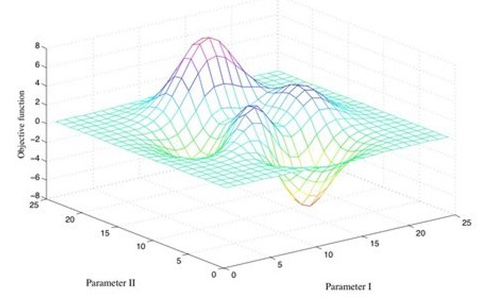
\includegraphics[scale=0.75]{grid.png}
\caption{Prikaz različitih kombinacija vrednosti atributa u vidu tačaka mreže}
\label{fig:slika1}
\end{figure}

\textbf{Slučajna pretraga} (eng. random search). Parametri se generišu slučajnim izborom.

\section{Performanse}
\label{sec:performanse}
Optimizovanje programa u okviru statičke kompilacije se zasniva na proceni poboljšanja 
bez prethodnog izvršavanja programa (različiti redosledi optimizacija daju različite rezultate). 
Odluka da nekoj transformaciji treba dati prednost u odnosu na drugu, kod statičke kompilacije,
donosi se na osnovu predefinisanog skupa ocena. Lako je zaključiti da primenom iterativne kompilacije 
možemo da testiramo veći broj mogućih nizova transformacija čime dolazimo do rešenja koja bolje optimizuju
program. 

\par
Tokom pretrage u okviru iterativne kompilacije kao glavni način ocenjivanja kvaliteta dobijenog niza transformacija
 se uzima vreme izvršavanja tako optimizovanog programa. Međutim, nama nije zabranjeno da pored vremena izvršavanja
 uvedemo još neke ocene kao na primer potrošnja energije. [Promeniti]Uvođenjem potrošnje enerije kao još jedne ocene kvaliteta,
  ne samo da tražimo rešenje koje nam daje najbolje vreme izvršavanja već i rešenje koje će nam samnjiti utrošak energije.

\subsection{Uticaj na vreme izvršavanja}
\label{sec:uticaj}
  Ovde ćemo izneti rezultate dobijene u \cite{kisuki2000iterative} koji prikazuju uticaj iterativne kompilacije 
 na brzinu izvršavanja programa i porede je sa brzinom programa koji je preveden statičkim metodom kompilacije.
\newline Tehnike optimizacije koje su korišćene:
\begin{enumerate}
\item Podela na blokove, gde su veličine blokova od 1 do 100;
\item Odmotavanje petlje, gde je faktor odmotavanja od 1 do 20;
\item Popunjavanje niza, gde je veličina popunjavanja od 1 to 10;
\end{enumerate}
Reperi koji su korišćeni za testiranje:
\begin{enumerate}
\item Množenje matrica (MxM), veličine podataka 256, 300 i 301;
\item Množenje matrica i vektora (MxV), veličine podataka 2048, 2300 i 2301;
\item Metod relaksacije (eng. \emph{Successive over-relaxation}, SOR), veličine podataka 128, 150 i 151;
\item Direktna diskretna kosinusna transformacija (eng. \emph{Forward Discrete Cosine Transform}, FDCT), veličine podataka 256, 300 i 301;
\item Rutina za kompenzaciju pokreta (eng. \emph{Motion compensation rutine}, RECO), veličine podataka 2048, 2300 i 2301;
\end{enumerate}
Programi su prevođeni na dva načina.
Prvi način prevođenja je takav da se pretraga u okviru iterativne kompilacije izvršava na 
fiksiranoj veličini ulaznih podataka. Prevođenje je rađeno odvojeno nad dva skupa
optimizacionih tehnika. Prvi skup čine tehnike 1. i 2. a drugi skup sve tri tehnike. Poboljšanje performansi 
tako prevedenih programa je prikazano na slikama \ref{fig:slika2} gde je korišćen prvi skup optimizacionih tehnika i 
\ref{fig:slika3} gde je korišćen drugi skup optimizacionih tehnika. Iz rezultata prikazanih na slici \ref{fig:slika2} vidimo da
je došlo do poboljšanja u brzini izvršavanja čak i do 3.4 puta. Možemo primetiti i da pretraga pronalazi 
dobro rešenje veoma brzo, unutar 50 iteracija u svim slučajevima ubrzanje programa je blizu maksimuma, osim
 u slučaju MxM i SOR. Kod MxM i SOR se tek nakon više od 100 iteracija dolazi do značajnog poboljšanja.
Ako uporedimo rezultate sa slike \ref{fig:slika2} i slike \ref{fig:slika3} vidimo da se približno ista poboljšanja
 dobijaju u okviru istog broja iteracija iako se korišćenjem drugog skupa optimizacija povećava prostor 
pretrage. U slučaju MxV se nakon 350 iteracija dobija bolje rešenje u odnosu na rešenje dobijeno korišćenjem prvog skupa 
optimizacija.

\begin{figure}[p]
\begin{center}
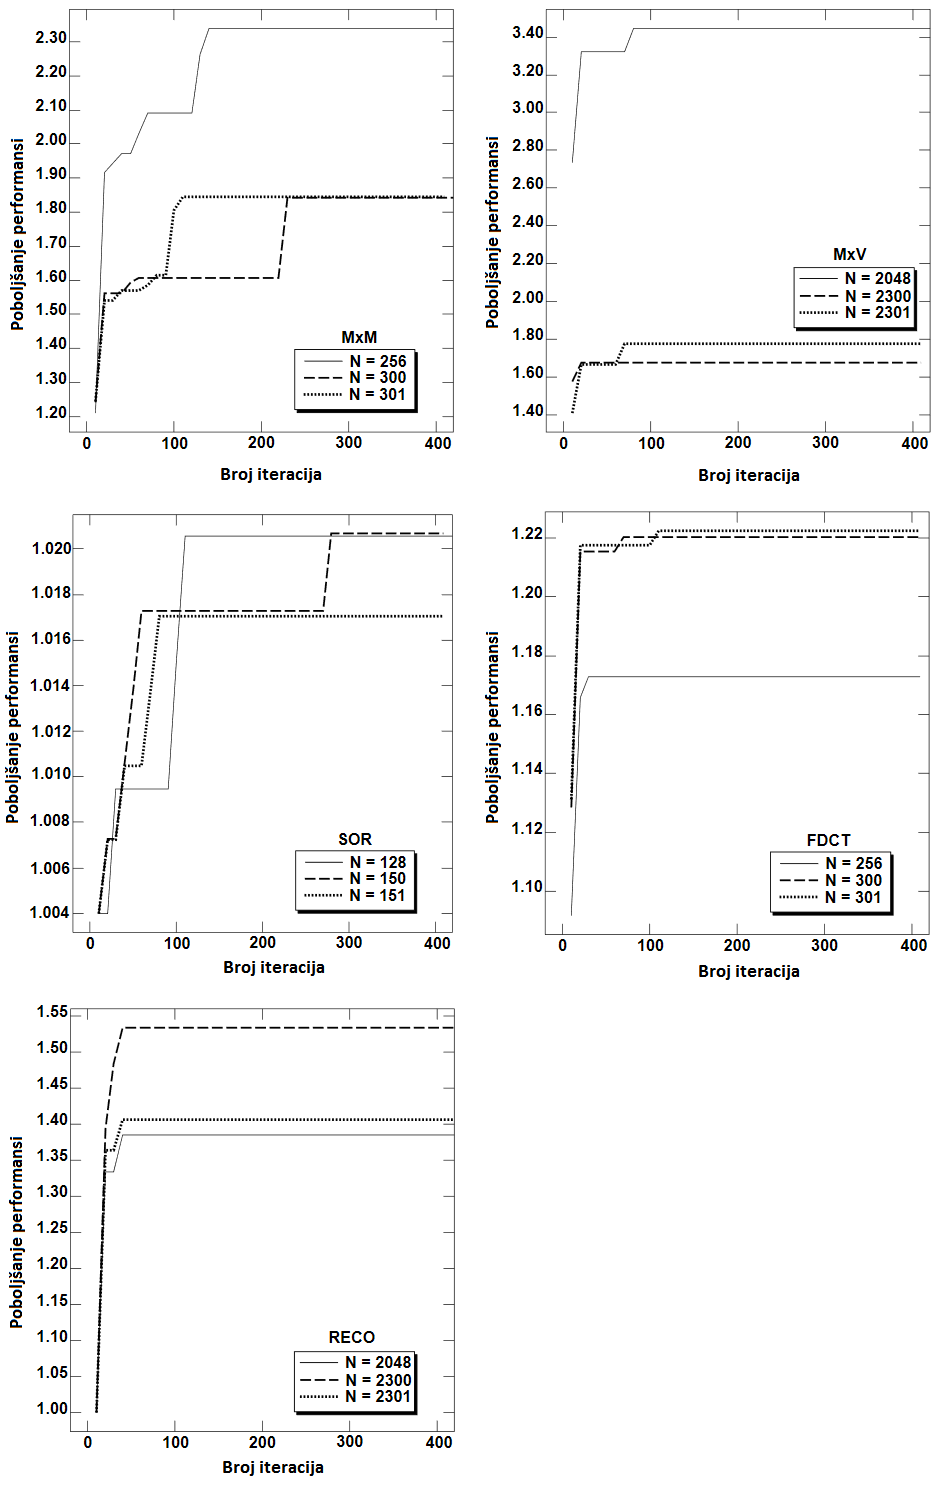
\includegraphics[width=\textwidth]{performanse1}
\end{center}
\caption{Poboljšanje performansi korišćenjem Odmotavanja i Podele na blokove}
\label{fig:slika2}
\end{figure}

\begin{figure}[p]
\begin{center}
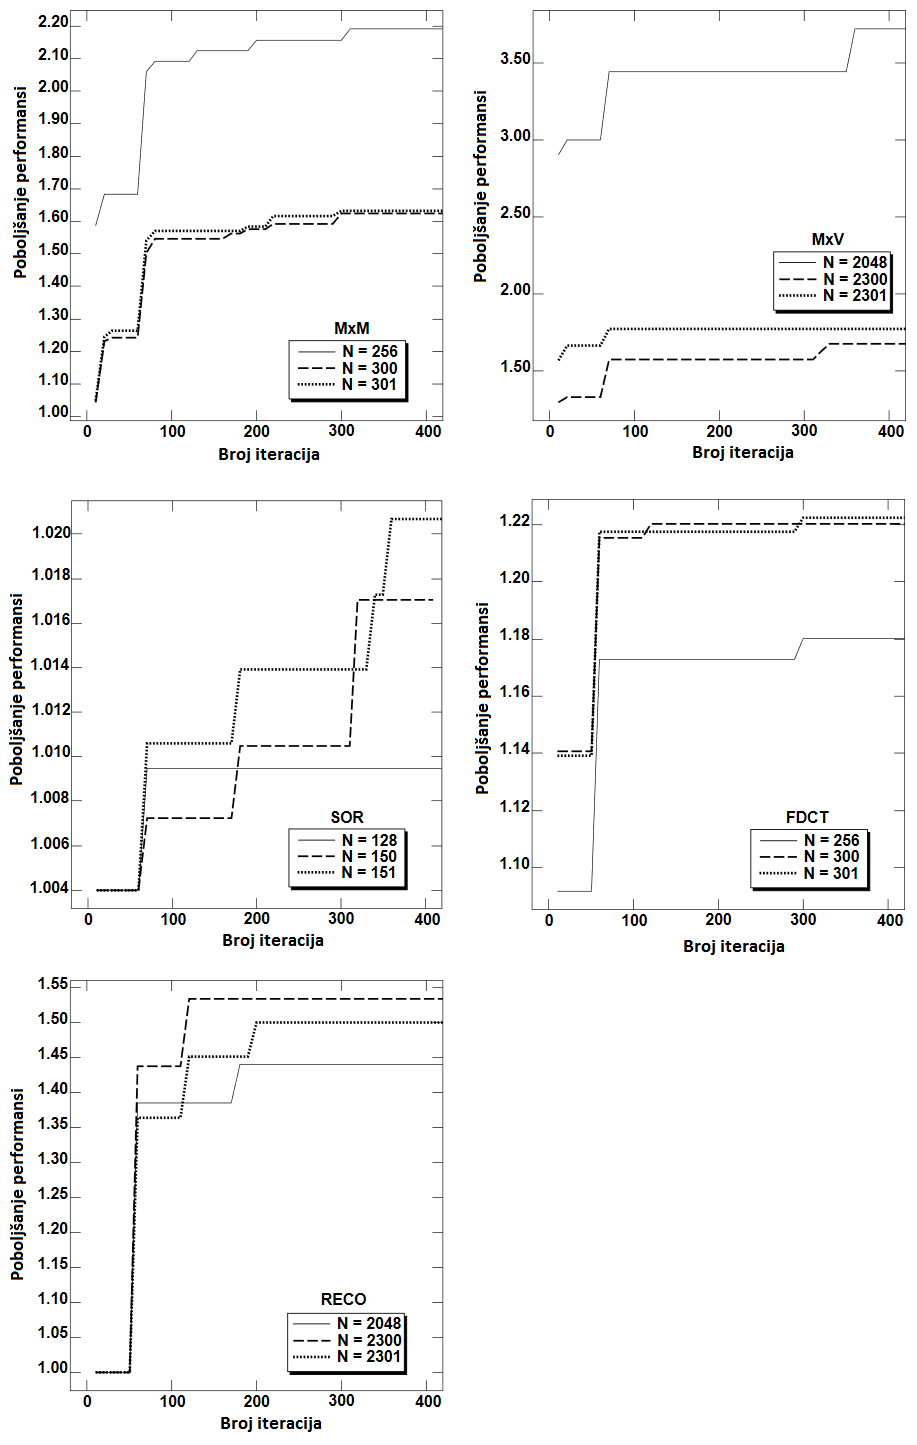
\includegraphics[width=\textwidth]{performanse2}
\end{center}
\caption{Poboljšanje performansi korišćenjem Odmotavanja, Podele na blokove i Popunjavanja niza}
\label{fig:slika3}
\end{figure}

Prvi način prevođenja je pokazao da su za fiksiranu veličinu ulaznih podataka preformanse dobijenih programa značajno poboljšane.
U praksi naš program se neće izvršavati stalno nad ulaznim podacima koji su iste veličine kao i oni koji su korišćeni 
pri kompilaciji, pa se iz tog razloga pristupilo i drugom načinu kompilacije. Kod drugog načina kompajliranja 
koriste se sve tehnike transformacije, a reperi koji se koriste za testiranje su MxM, MxV, FDCT i RECO.
Pretraga u okviru kompilacije će se izvršavati nad više različitih ulaznih podataka gde će se kao mera kvaliteta uzimati
srednja vrednost dobijenih rezultata. Na slici \ref{fig:slika4} prikazani su dobijeni rezultati.
Crnom bojom su prikazani rezultati dobijeni prvim načinom kompilacije. Sivom bojom su prikazani rezultati dobijeni
drugim načinom kompilacije, s tim što su veličine ulaznih podataka sledeće:
\begin{itemize}
\item 256, 300 i 301 za MxM i FDCT
\item 2048, 2300 i 2301 za MxV i RECO
\end{itemize}
Belom bojom su prikazani rezultati dobijeni drugim načinom kompilacije, a veličine ulaznih podataka su:
\begin{itemize}
\item 250, 260, 290 i 310 za MxM i FDCT
\item 2000, 2100, 2200, 2400 za MxV i RECO
\end{itemize}
Svaki dobijeni program je pokrenut na reperima čije su veličine definisane na početku ove sekcije.
Ako pogledamo grafik videćemo da rezultati dobijeni drugom metodom kompilacije i dalje daju značajna poboljšanja 
u brzini izvršavanja. Možemo primetiti i da je brzina izvršavanja programa dobijenih drugom metodom za nijansu 
sporija od programa dobijenih prvom metodom. U slučaju MxM vidimo da je program kompajliran sa 3 različite veličine 
ulaznih podataka brži od programa koji se dobija prilikom prevođenja sa fiksiranom veličinom ulaza.

\begin{figure}[h]
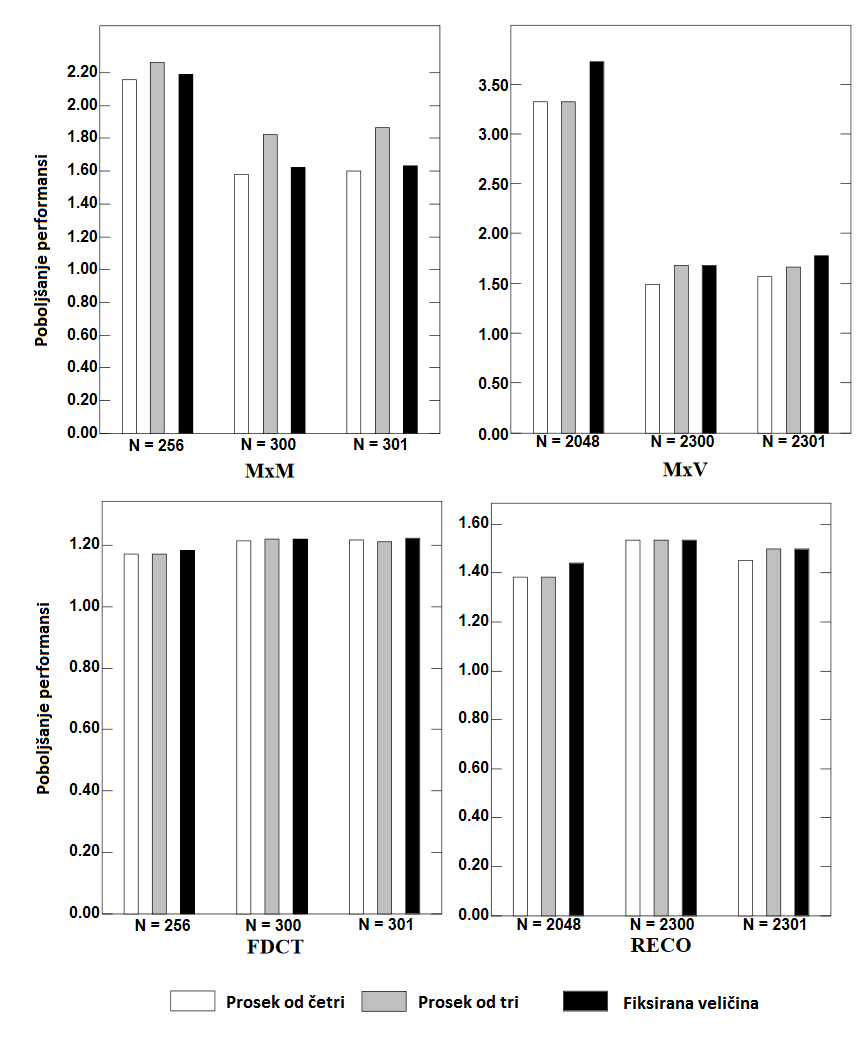
\includegraphics[scale=0.5]{performanse3}
\caption{Poredjenje poboljšanja performansi}
\label{fig:slika4}
\end{figure}

\subsection{Odnos vremena izvršavanja i uštede energije}
\label{sec:naslov}
Transformacije koje se koriste za optimizaciju pored toga što utiču na poboljšanje vremena izvršavanja,
 takođe utiču i na potrošnju energije. Kao što su različiti nizovi transformacija različito uticali na vreme izvršavanja, 
 tako različiti nizovi transformacija utiču i na potrošnju. Na osnovu iznetih informacija u prethodnim sekcijama možemo 
 pomisliti da niz transformacija koji daje rešenje sa najboljim vremenom izvršavanja
 ujedno daje i rešenje sa najvećom uštedom energije. Takav zaključak je ispravan u većini slučajeva.
\par
Da bismo potkrepili prethodnu priču iznećemo neke praktične rezultate koje su prikazani u \cite{gheorghita2005iterative}.
Prikazaćemo rezultate koji su dobijeni nad reperima MxM (veličine 128) i SOR (veličine 512). Od transformacija 
su korišćene odmotavanje petlji (sa faktorom odmotavanja između 0 i 40) i podela na blokove (sa veličinom bloka između 0 i 100).
Za svaki par parametara je pronadjeno rešenje i izemeereno vreme izvršavanja i potrošnja energije, a zatim su se dobijeni rezultati 
uporedili sa najboljim mogućim rešenjem. Rezultati su prikazani na slici \ref{fig:slika5}. 
Grafikoni pod a i c predstavljaju odnos između vremena izvršavanja dok grafikoni pod b i d odnos između potrošnje energije.
Svaka od boja predstavlja odnos koliko je dobijeno rešenje gore od najboljeg i to u procentima. 
Značenje svake od boja je prikazano u tabeli \ref{tab:tab1}.

\par
Ako pogledamo grafikone vidimo da se oblasti koje daju najmanje odstupanja kako u vremenu izvršavanja tako i u uštedi energije poklapaju
kao i da rešenja koja odstupaju u vremenu iz u performansama takođe mogu da budu optimalna što se tiče uštede energije.

\begin{figure}[p]
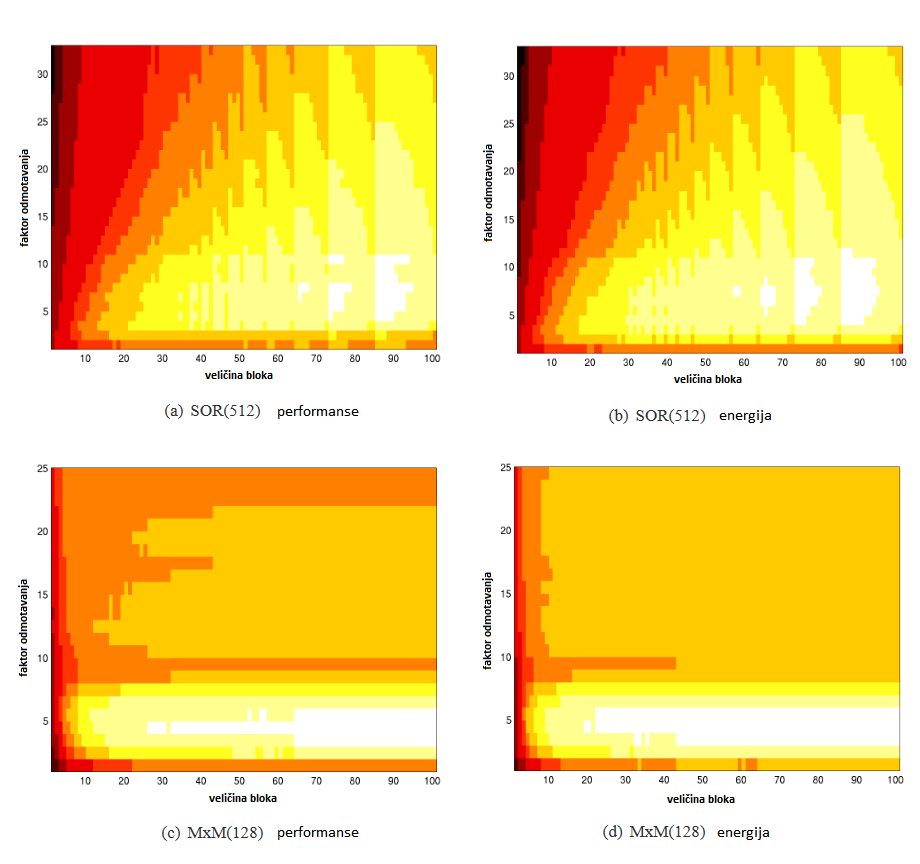
\includegraphics[scale=0.5]{performanse4}
\caption{Prikaz dobijenih rezltata za MxM i SOR}
\label{fig:slika5}
\end{figure}

\begin{table}[]
\centering
\caption{Predložiti naslov}
\label{tab:tab1}
\begin{tabular}{|c|l|c|l|l|}
\hline
\multicolumn{2}{|c|}{Boja}                     & \multicolumn{3}{l|}{Koliko je rešenje lošije od najboljeg mogućeg} \\ \hline
\multicolumn{2}{|c|}{\cellcolor[HTML]{FFFFFF}} & \multicolumn{3}{c|}{Između 0\% - 3\%}                              \\ \hline
\multicolumn{2}{|c|}{\cellcolor[HTML]{FFFF8F}} & \multicolumn{3}{c|}{Između 3\% - 10\%}                             \\ \hline
\multicolumn{2}{|c|}{\cellcolor[HTML]{FEFF1F}} & \multicolumn{3}{c|}{Između 10\% - 17\%}                            \\ \hline
\multicolumn{2}{|c|}{\cellcolor[HTML]{FFCA00}} & \multicolumn{3}{c|}{Između 17\% - 25\%}                            \\ \hline
\multicolumn{2}{|c|}{\cellcolor[HTML]{FF7F00}} & \multicolumn{3}{c|}{Između 25\% - 35\%}                            \\ \hline
\multicolumn{2}{|c|}{\cellcolor[HTML]{FE3500}} & \multicolumn{3}{c|}{Između 25\% - 50\%}                            \\ \hline
\multicolumn{2}{|c|}{\cellcolor[HTML]{EA0001}} & \multicolumn{3}{c|}{Između 50\% - 100\%}                           \\ \hline
\multicolumn{2}{|c|}{\cellcolor[HTML]{9F0100}} & \multicolumn{3}{c|}{Između 100\% - 200\%}                          \\ \hline
\multicolumn{2}{|c|}{\cellcolor[HTML]{540000}} & \multicolumn{3}{c|}{Između 200\% - 300\%}                          \\ \hline
\multicolumn{2}{|c|}{\cellcolor[HTML]{0A0000}} & \multicolumn{3}{c|}{Preko 300\%}                                   \\ \hline
\end{tabular}
\end{table}

\newpage
\section{Zaključak}
\label{sec:zakljucak}
U ovom radu opisali smo tehniku iterativne kompilacije. 
Pokazali smo da ova tehnika u mnogim situacijama dovodi 
do značajnih ubrzanja i da su u gotovo svim situacijama 
programi optimizovani iterativnom kompilacijom značajno 
brži od programa kompajliranih statičkim metodama, kao i da koriste
značajno manje energije.
\par
Na osnovu načina traganja za najboljim transformacijama 
i najboljim ulaznim parametrima za te optimizacije možemo da zaključimo
da iako je izvršavanje programa prevedenih ovom tehnikom brže
od statički prevedenih ekvivalenata, sam čin prevođenja je značajno sporiji. 
Upravo zbog toga ovaj metod prevođenja nije pogodan za vreme samog
razvijanja softvera, 
ali je više nego poželjan za primenu na verzijama softvera prevedenih 
i spremljenih za isporuku.
\par
Značaj ove tehnike može imati izuzetnog uticaja
na efikasnost uređaja u svetu \emph{interneta stvari} (eng. \emph{Internet Of Things}) 
gde većina uređaja ima ograničenu dostupnost električne energije, kao i u svetu 
mobilnih uređaja.
\par
Nadamo se da će sa kompajlerima koji se budu razvijali u budućnosti u paketu 
dolaziti i mnoge optimizacione tehnike i alati među kojima ćemo videti i
neke varijante iterativne kompilacije.
\addcontentsline{toc}{section}{Literatura}
\appendix
\bibliography{seminarski} 
\bibliographystyle{plain}

\end{document}
